\chapter{STUDY III - INNER SIDE DIAGNOSIS IMPROVEMENT }\label{chp:Inner Side Diagnosis Improvement}

This chapter is focused on arch high index calculation improvements with the data provided in Chapter \ref{chp:Back Side Diagnosis}. In this study, analysis and design decisions in Section \ref{sec:StudyIIIAnalysisAndDesign}, specifics of implementation in Section \ref{sec:StudyIIIImplementation}, and initial test findings and evaluation phase in Section \ref{sec:StudyIIITestAndEvaluation} will be discussed.

\section{ANALYSIS AND DESIGN}\label{sec:StudyIIIAnalysisAndDesign}

Preliminary detection of potential pes planus and pes cavus patients will be provided based on the inner side photographs of the foot. This system will be based on the initial implementation of the arch height index calculation discussed in Chapter \ref{chp:Foot Detection & Primary Diagnosis}. In addition, this chapter profoundly focuses on improving the batch process on pre-diagnosis.

Three major fallbacks of the initial design are discovered in the test end evaluation of the process. All the fallbacks and potential solutions were discussed in the following paragraphs.

The first fallback is the differences between the line of the sole and the symmetry of the foot sole function. These differences should be reduced, and the foot function's sole should be more accurate.

The second fallback is that the bottom of the images contains a lot of noise in edge detection. By eliminating these noises, the accuracy of the foot sole function should be increased. The greedy approach could be used to improve accuracy with a relatively less computational resource.

The third fallback is that there is no error detection mechanism to reduce the error. Therefore, the function of the foot sole should not only be used for point detection but also for detecting the slope of the foot. As a result, this feature extraction should be used for detecting anomalies so that the results can be corrected.

\section{IMPLEMENTATION}\label{sec:StudyIIIImplementation}

Implementation details of the changes in the batch process will be discussed separately in this section.

\begin{figure}[htbp]
\centering
\fbox{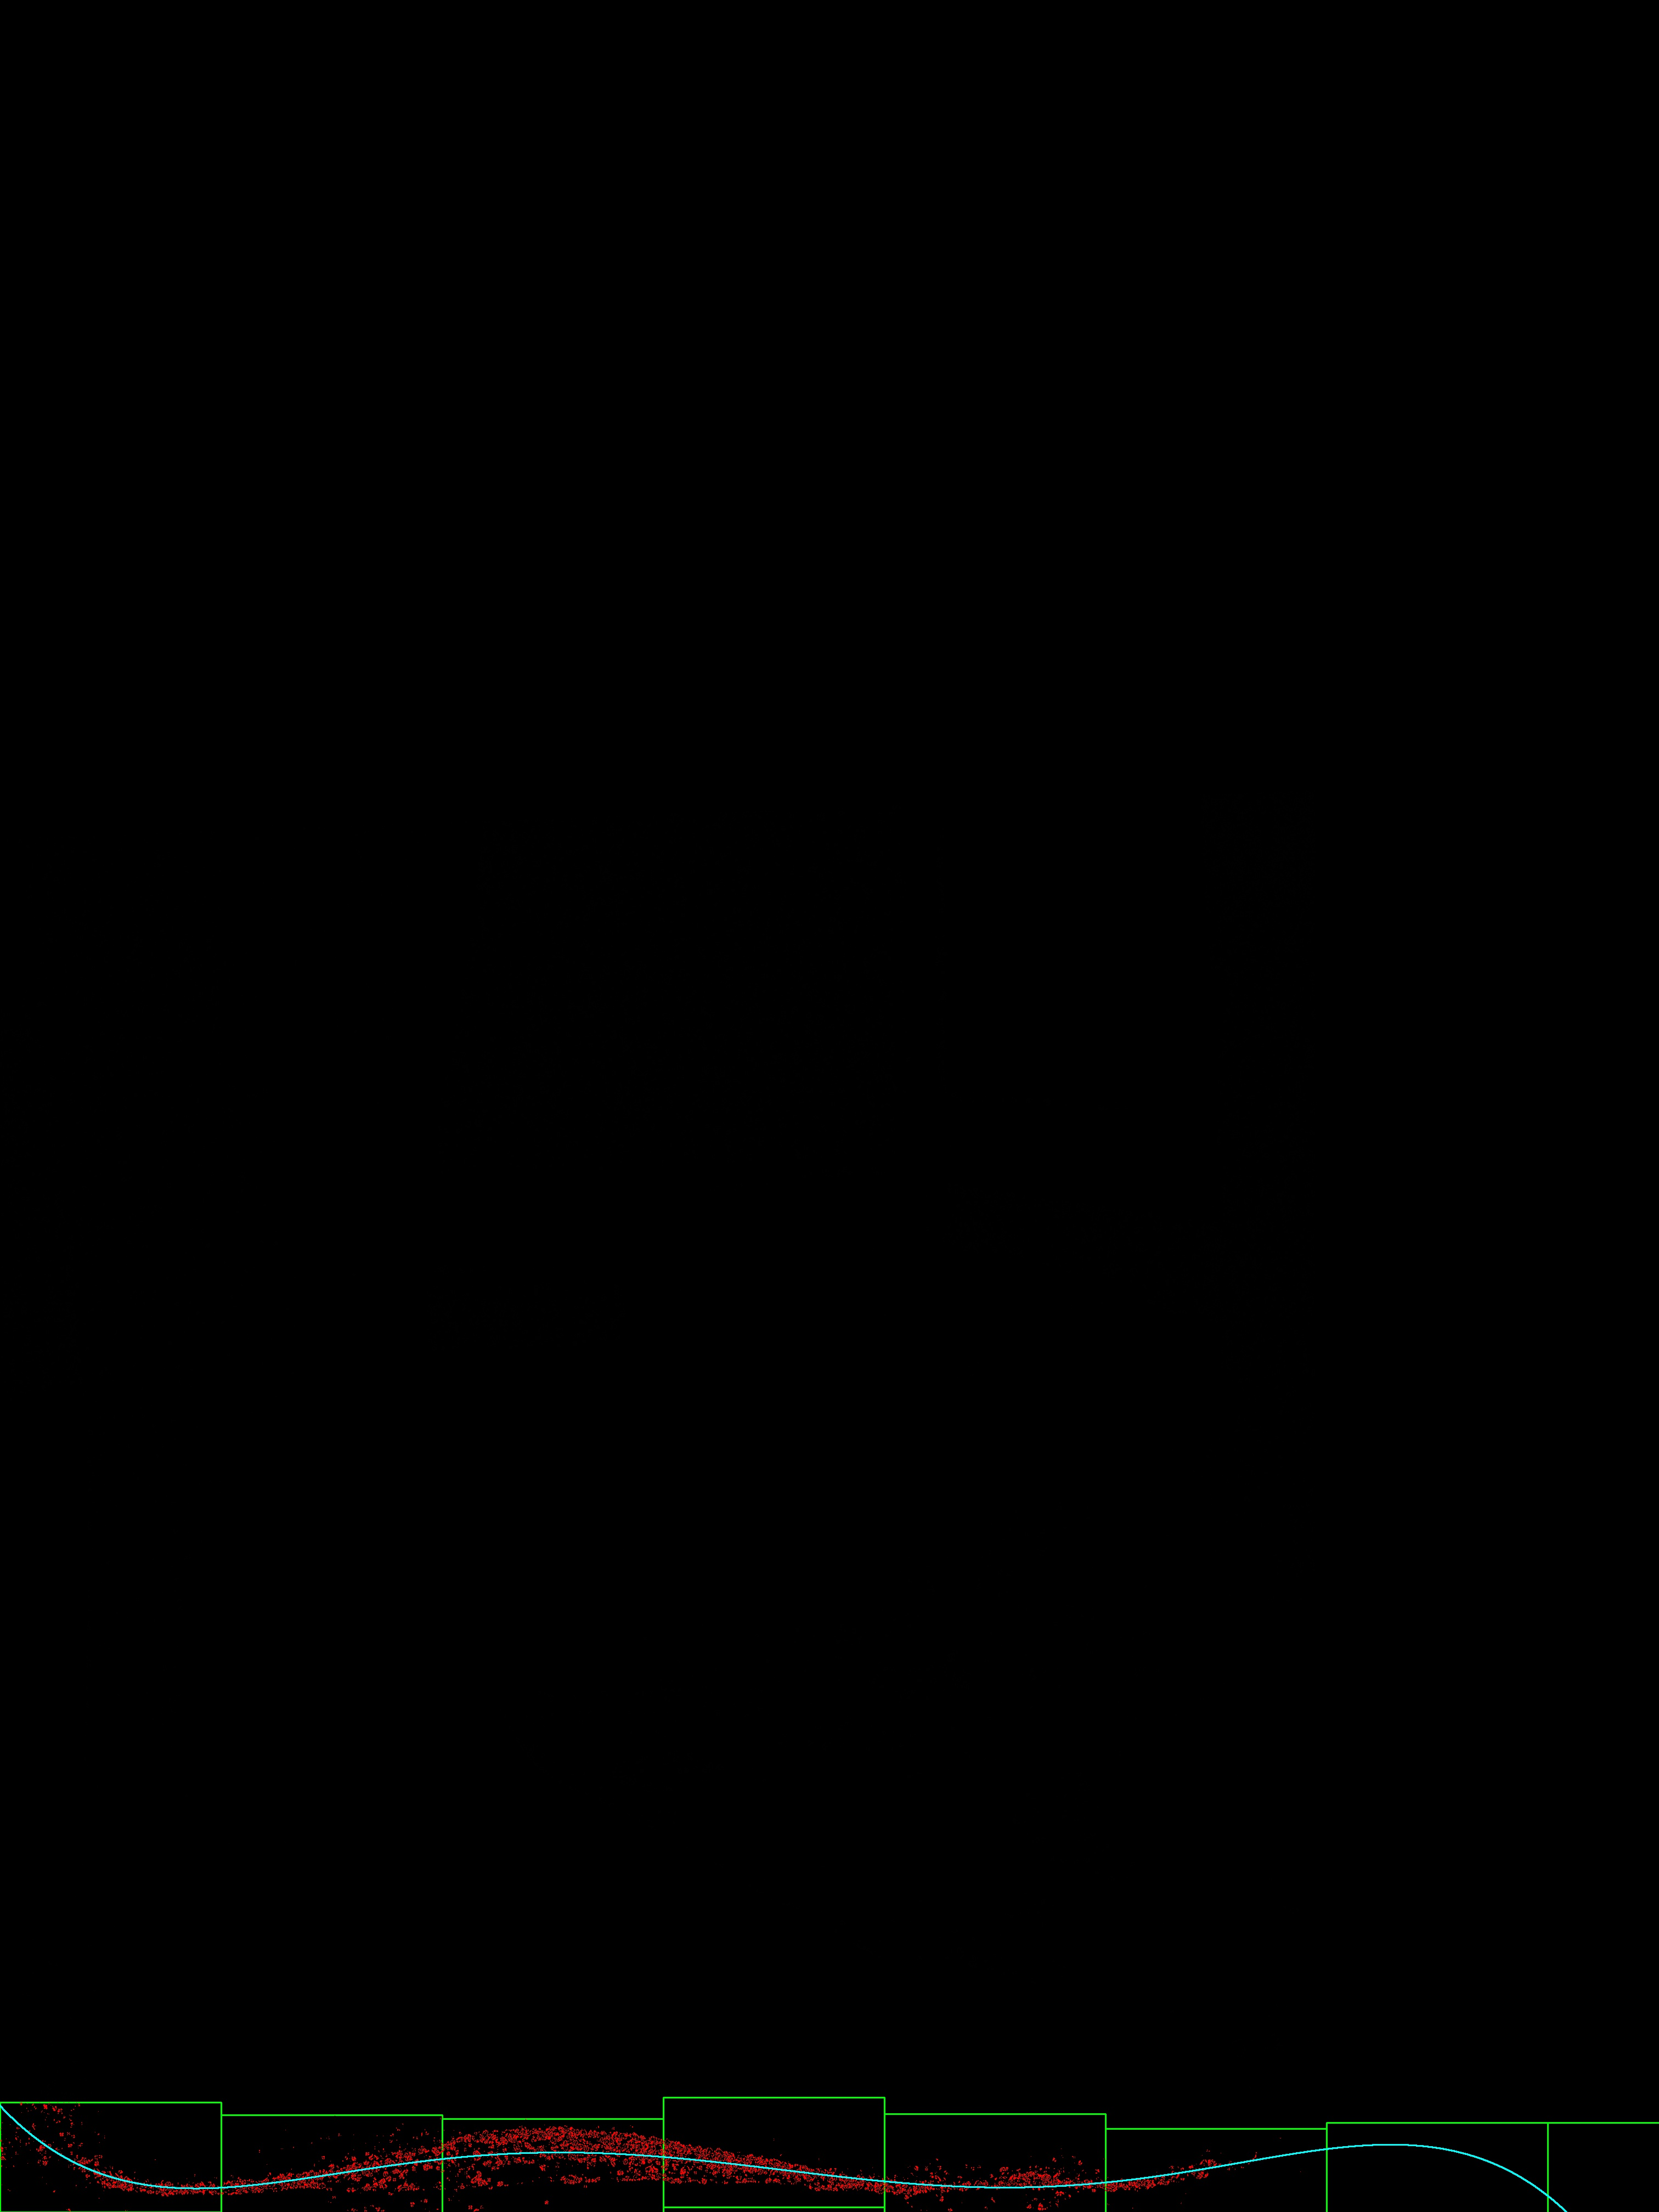
\includegraphics[width=.60\columnwidth]{KaanEksenMSc/figures/StudyIIIPredefinedWindows.jpeg}}
\caption{Accuracy improvement with polynomial regression window in study III}
\label{fig:StudyIIIPredefinedWindows}
\end{figure}

The first fallback is the accuracy of the foot sole function. The foot sole function calculation was designed to reduce the sudden slope changes to the function because there might be an error in edge detection. Increasing the predefined windows, where polynomial regression is applied, will improve the function’s response to changes (see Figure \ref{fig:StudyIIIPredefinedWindows}).

\begin{figure}[htbp]
\centering
\fbox{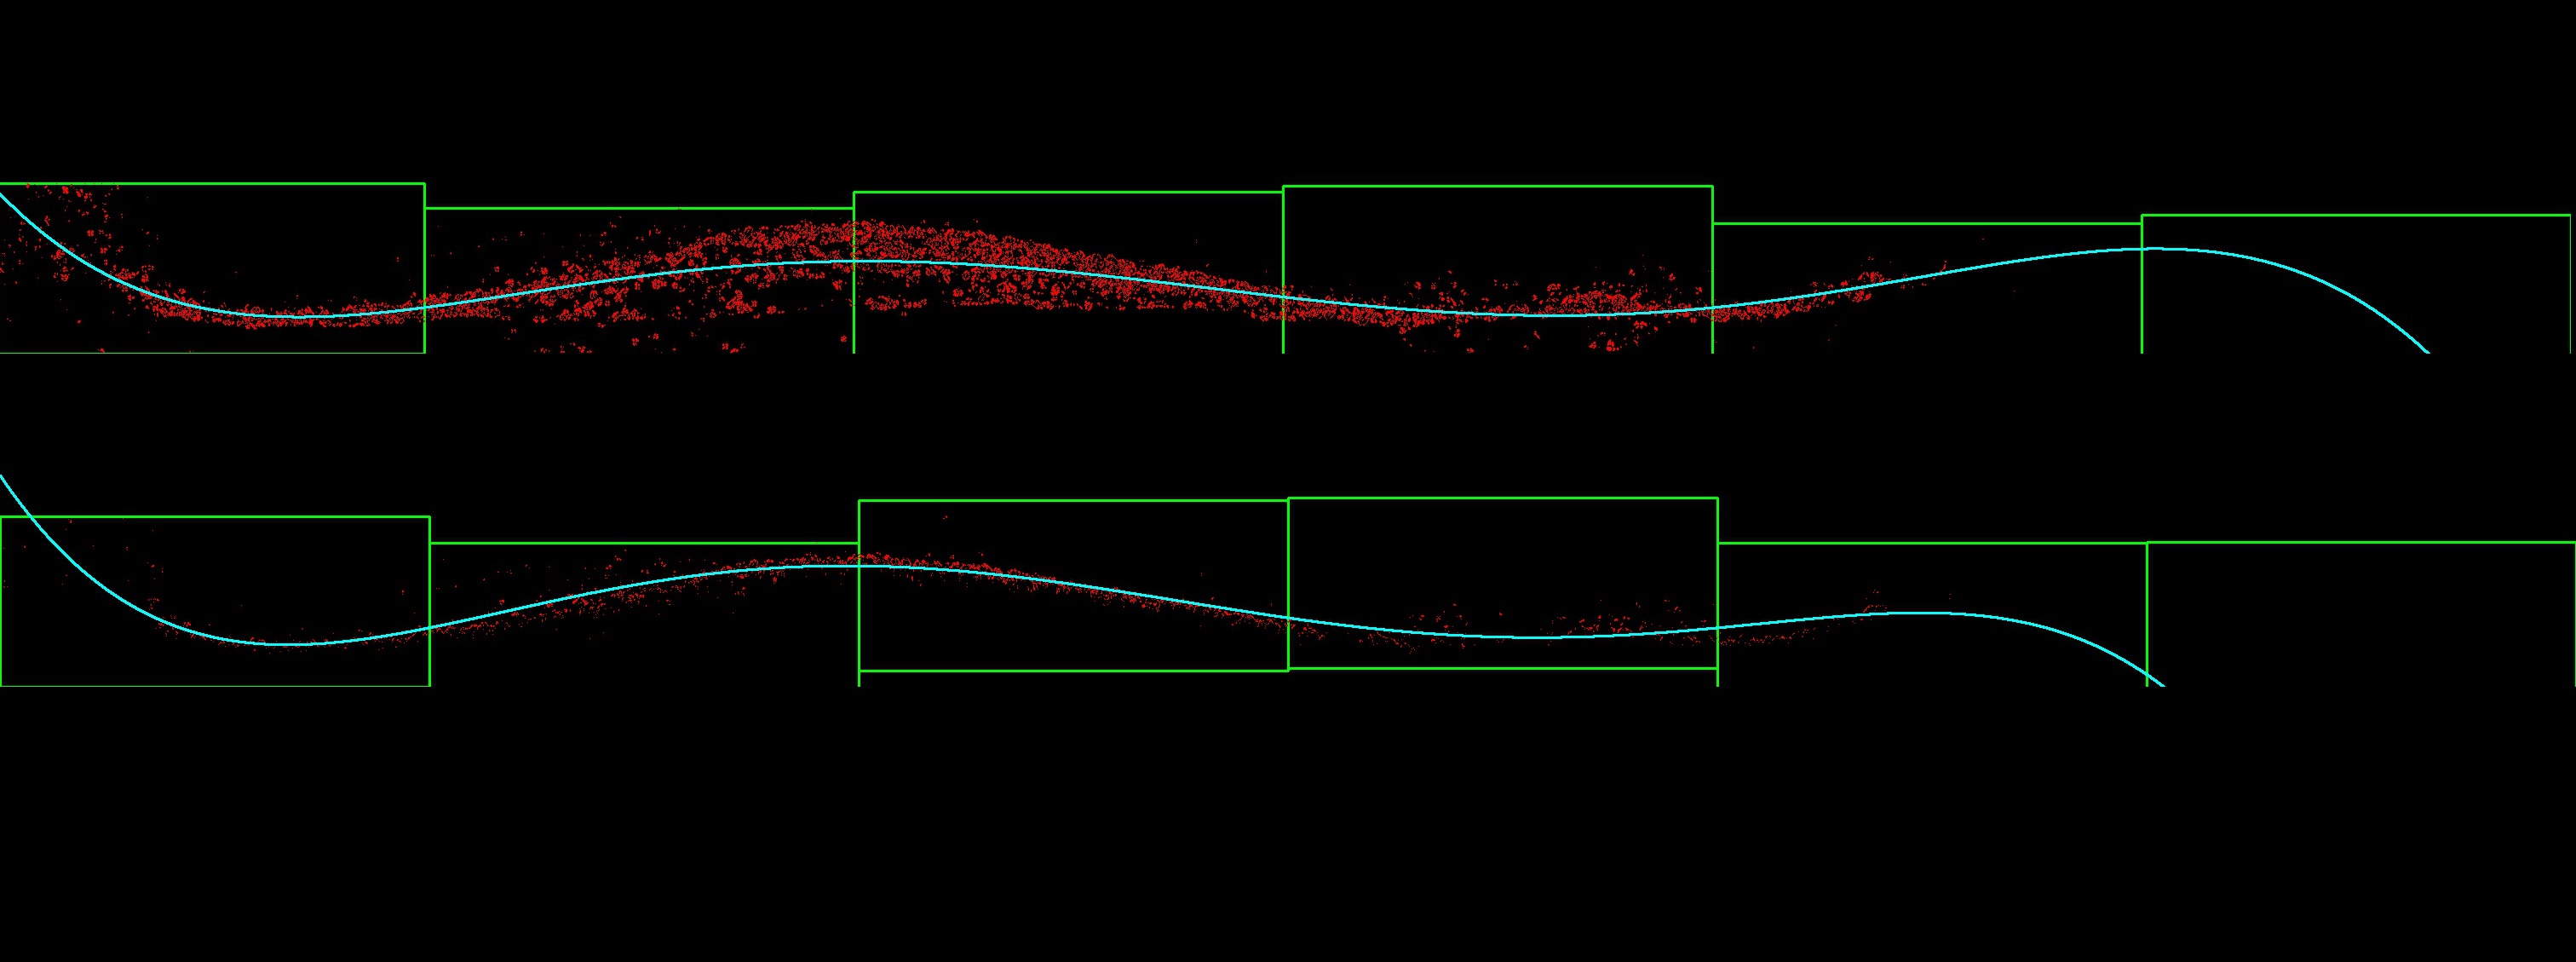
\includegraphics[width=.80\columnwidth]{KaanEksenMSc/figures/StudyIIINoiseReduce.jpg}}
\caption{Greedy noise reduce improvement in study III}
\label{fig:StudyIIINoiseReduce}
\end{figure}

The second fallback is that the edge images contain noise. Since the bottom of the image edge points changes according to the floor decoration (carpet, faience etc.), removing the edge points of the floor will significantly improve the accuracy of the foot sole function. Since there is no edge point across the foot surface, greedy approach was used to removing the bottom edge points (see Figure \ref{fig:StudyIIINoiseReduce}). In addition, removing 80 percent of the dots in each row was resulted in the best accuracy in the tests.

\begin{figure}[htbp]
\centering
\fbox{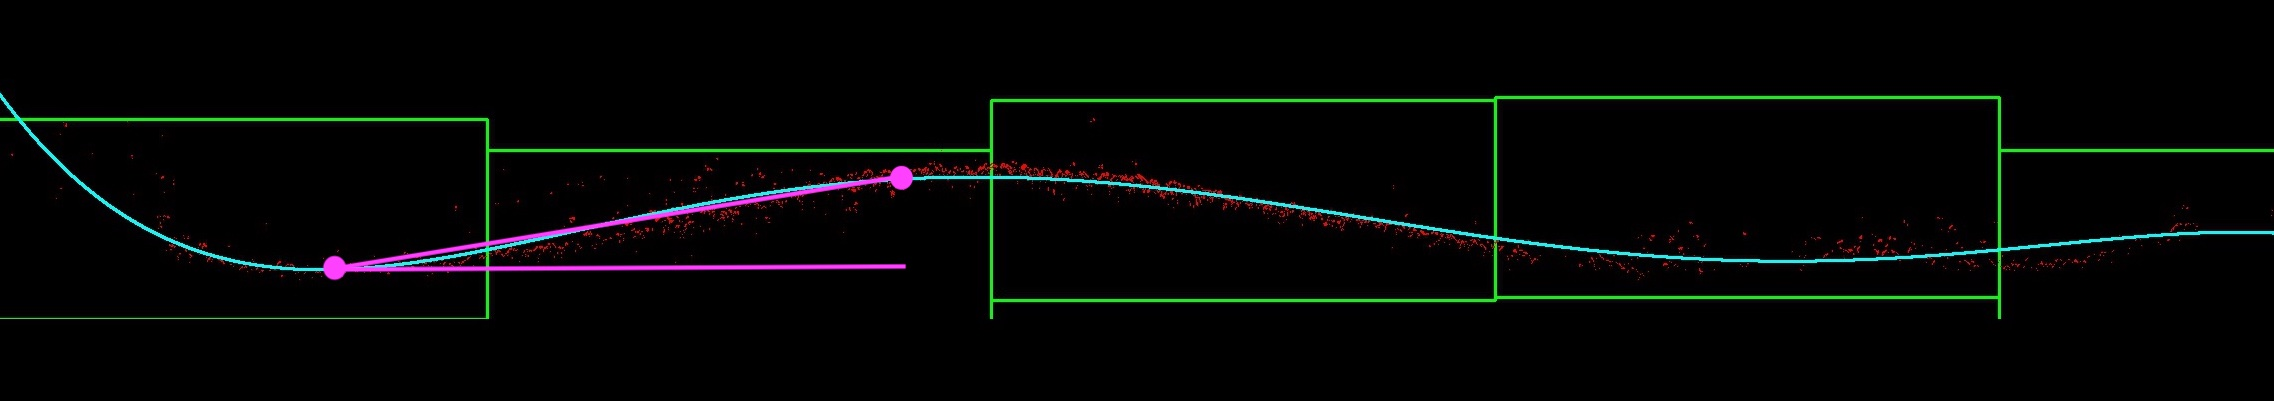
\includegraphics[width=.80\columnwidth]{KaanEksenMSc/figures/StudyIIISlopeCalculation.jpg}}
\caption{Slope calculation for error detection mechanism  in study III}
\label{fig:StudyIIISlopeCalculation}
\end{figure}

The final fallback is the lack of an error detection mechanism. If the slope is higher than a certain rate, it is an indication of pes cavus. Likewise, the same assumption can be made for the low slope. Therefore, with the improved foot sole function, error detection mechanism was obtained by calculating the slope of the function at certain positions. Error detection mechanism was implemented by taking two points on the foot; as the heel's peak and the foot space in the center (see Figure \ref{fig:StudyIIISlopeCalculation}).

\section{TEST AND EVALUATION}\label{sec:StudyIIITestAndEvaluation}

In this section, the testing and evaluation process of the prototype system, which is explained in detail in the previous sections, will be discussed. There is no data collection part in this study; the data discussed in Section \ref{sec:StudyIITestAndEvaluation} were used. Therefore, data collection and data details will be skipped.

\begin{figure}[htbp]
\centering
\fbox{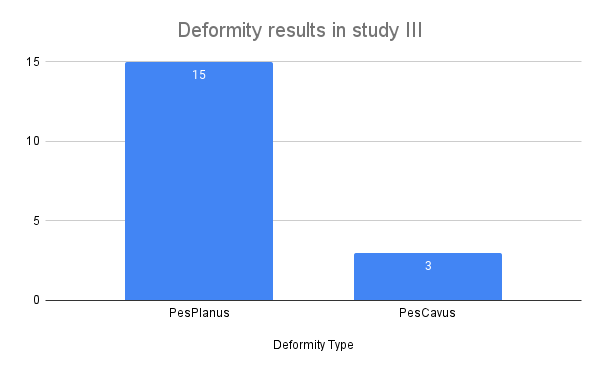
\includegraphics[width=.60\columnwidth]{KaanEksenMSc/figures/StudyIIIFootDeformityAutomatedProcessResults.png}}
\caption{Foot deformity distribution in automated process results in study III}
\label{fig:StudyIIIFootDeformityAutomatedProcessResults}
\end{figure} 

The findings of the healthcare officials and the system were matched 83,3 percent of the time (see Figure \ref{fig:StudyIIIFootDeformityAutomatedProcessResults}). One pes planus and two pes cavus mismatch in detection are recorded. Inner side diagnosis improvements were very promising (see Figure \ref{fig:StudyIIISlopeResults}). However, the test population was not diverse. Therefore the system should be tested on a larger population to get more accurate results.

\begin{figure}[htbp]
\centering
\fbox{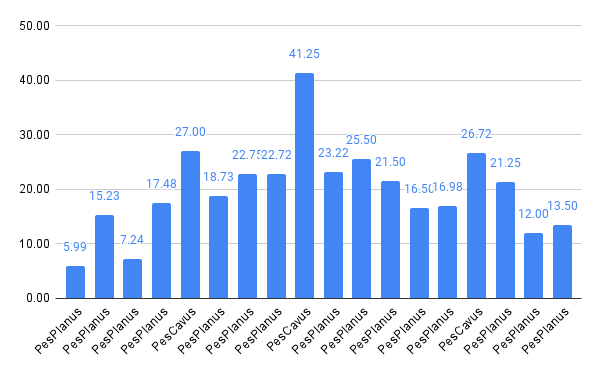
\includegraphics[width=.60\columnwidth]{KaanEksenMSc/figures/StudyIIISlopeResults.png}}
\caption{Foot deformity and calculated slope in automated process results in Study III}
\label{fig:StudyIIISlopeResults}
\end{figure} 

